\documentclass[11pt]{article}
\usepackage[margin=1in]{geometry}
\usepackage[T1]{fontenc}
\usepackage{lmodern}
\usepackage{microtype}
\usepackage{amsmath,amssymb,amsthm,mathtools}
\usepackage{booktabs,longtable,array}
\usepackage{enumitem}
\usepackage{graphicx}
\usepackage{xcolor}
\usepackage[hidelinks]{hyperref}
\usepackage{url}
\usepackage{listings}
\usepackage{fancyhdr}
\usepackage{caption}
\usepackage{subcaption}

\definecolor{codegray}{gray}{0.96}
\lstset{basicstyle=\ttfamily\small,backgroundcolor=\color{codegray},frame=single,
  breaklines=true,columns=fullflexible}
\setlength{\headheight}{14pt}
\pagestyle{fancy}
\fancyhf{}
\lhead{Aperiodic monotile in iPRA}
\rhead{16 November 2026}
\cfoot{\thepage}

\newtheorem{theorem}{Theorem}[section]
\newtheorem{lemma}[theorem]{Lemma}
\newtheorem{proposition}[theorem]{Proposition}
\newtheorem{corollary}[theorem]{Corollary}
\newtheorem{definition}[theorem]{Definition}
\newtheorem{remark}[theorem]{Remark}
\newtheorem{claim}[theorem]{Claim}
\newcommand{\iPRA}{\mathrm{iPRA}}
\newcommand{\PA}{\mathrm{PA}}
\newcommand{\N}{\mathbb N}
\newcommand{\Z}{\mathbb Z}
\newcommand{\Q}{\mathbb Q}
\newcommand{\Htile}{\mathsf H}
\newcommand{\code}[1]{\ulcorner #1\urcorner}
\newcommand{\normform}[2]{Q(#1,#2)}
\newcommand{\True}{\mathbf 1}
\newcommand{\False}{\mathbf 0}

\title{An Aperiodic Planar Monotile in Intuitionistic Primitive Recursive Arithmetic\\
\large A finitary certificate proof for the hat monotile}
\author{Research packet prepared for Vladimir Reshetnikov}
\date{16 November 2026}

\begin{document}
\maketitle

\begin{abstract}
We recast the existence and aperiodicity of the Smith--Myers--Kaplan--Goodman-Strauss
``hat'' monotile as a theorem of intuitionistic primitive recursive arithmetic
($\iPRA$).  The central point is that $\iPRA$ is a first-order arithmetic theory and
therefore does not literally quantify over subsets of the Euclidean plane.  We replace
that higher-order statement by an arithmetical certificate theorem with two parts:
(1) a primitive-recursive, coherent sequence of exact finite hat patches covers every
prescribed lattice ball, and (2) every finite code for a periodic quotient of a hat
tiling is rejected.  The first part is witnessed by the explicit four-metatile
substitution.  The second is a finite-torus form of the chevron/comet coupling proof:
area forces determinant $2/3$, strip cycles force the period map to be a similarity,
and the triangular-lattice norm
\[
  Q(m,n)=m^2+mn+n^2
\]
gives a constructive $2$-adic descent contradiction.  All geometric computations take
place over rational axial coordinates; all searches are bounded; and all inductions are
quantifier-free.  Thus the proof uses exactly the resources available in $\iPRA$.

The archive contains this report, exact certificate data, a standard-library Python
reference verifier, generated evidence, and a detailed Lean scaffold aimed at
\texttt{ConciseIPRA} and \texttt{IPRADerivations} in the ProveIt repository.  The Lean
files are an outline with explicit \texttt{sorry} obligations, not a completed
kernel-checked derivation.
\end{abstract}

\tableofcontents

\section{Result, scope, and formal status}

\subsection{The ordinary geometric theorem}
A planar monotile is a single compact topological disk whose congruent copies tile the
plane.  It is aperiodic if it tiles the plane but no such tiling has a nonzero
translational symmetry.  Smith, Myers, Kaplan, and Goodman-Strauss proved that the hat,
a polygonal union of eight congruent kites, is an aperiodic monotile.  We use their
explicit metatile construction for existence and their geometric coupling argument for
nonperiodicity.

\begin{theorem}[Geometric hat theorem]\label{thm:geometric}
There is a polygon $\Htile\subset\mathbb R^2$ such that
\begin{enumerate}[label=(\roman*)]
\item the plane is a union of pairwise interior-disjoint congruent copies of $\Htile$;
\item no tiling by congruent copies of $\Htile$ is invariant under a nonzero translation.
\end{enumerate}
\end{theorem}

The difficulty in asking for Theorem~\ref{thm:geometric} ``in $\iPRA$'' is logical, not
geometric.  The language of $\iPRA$ has only natural-number variables.  It cannot form a
single internal variable ranging over an arbitrary infinite set of real polygons.  A
faithful arithmetic formulation must therefore say what finite observations and finite
obstructions constitute a tiling.

\subsection{The arithmetical theorem}
Fix primitive-recursive codings of signed integers, pairs, finite lists, rational affine
maps, polygons, finite patches, and finite torus quotients.  Let
\begin{align*}
 \mathsf{PatchOK}(p)&\in\{0,1\},\\
 \mathsf{Covers}(p,r)&\in\{0,1\},\\
 \mathsf{TorusHat}(c)&\in\{0,1\}
\end{align*}
be the exact Boolean predicates defined in Section~\ref{sec:coding}.  The first checks
that $p$ is a gap-free, overlap-free finite patch of hats.  The second checks that $p$
covers the axial hexagon of radius $r$.  The third checks a finite periodic quotient:
two independent period vectors, finitely many tile representatives, and all local
incidence conditions modulo their period lattice.

Let $P(n)$ be the primitive-recursive nested $H$-supertile patch of level $n$, and let
$R(n)$ be its certified radius.  The internal sentence is
\begin{equation}\label{eq:internal}
\mathsf{Einstein}_{\Htile}\;\equiv\;
\left[\forall r\;\exists n\,
   (r\le R(n)\wedge \mathsf{PatchOK}(P(n))=1
       \wedge \mathsf{Covers}(P(n),r)=1)\right]
\wedge
\left[\forall c\;\mathsf{TorusHat}(c)=0\right].
\end{equation}
Every symbol in~\eqref{eq:internal} denotes a primitive-recursive function.  Formula
\eqref{eq:internal} is consequently an ordinary first-order arithmetic sentence.

\begin{theorem}[iPRA certificate theorem]\label{thm:ipra}
Intuitionistic primitive recursive arithmetic proves
\[
   \iPRA\vdash \mathsf{Einstein}_{\Htile}.
\]
More precisely, after expanding the primitive-recursive symbols by their defining
equations, the proof uses intuitionistic first-order logic, equality, successor axioms,
and induction only for quantifier-free formulas.
\end{theorem}

\begin{remark}[What is, and is not, internal]
The left conjunct of~\eqref{eq:internal} is stronger than a mere assertion that every
radius is separately tileable: the patches are values of one fixed primitive-recursive
program and are coherent under restriction.  Externally their union is therefore an
explicit computable tiling, with no appeal to a nonconstructive compactness theorem.
The right conjunct is exactly the finite object that a strongly periodic tiling would
supply.  Lemmas~\ref{lem:weakstrong} and~\ref{lem:alignment} show constructively that a
weakly periodic hat tiling would supply such a torus code.  Thus
Theorem~\ref{thm:ipra}, under the standard interpretation of the codes, yields
Theorem~\ref{thm:geometric}.
\end{remark}

\subsection{Audit status}
The mathematical reduction and the human proof are complete at the certificate level.
The delivered Python program checks the closed hat data, the substitution counts, the
key exact rational geometry for six generations, and the arithmetic obstruction.  The
Lean directory gives all definitions and a dependency-complete route to a kernel proof,
but still contains explicit \texttt{sorry} declarations.  In particular, this packet
does not claim that \texttt{einstein\_hat\_ipra} has already been accepted by Lean.

\section{Exact geometry and primitive-recursive coding}\label{sec:coding}

\subsection{The triangular lattice}
Let
\[
 e_0=(1,0),\qquad e_1=\left(\frac12,\frac{\sqrt3}{2}\right).
\]
An axial pair $(u,v)\in\Z^2$ denotes $u e_0+v e_1$.  Its squared Euclidean norm is
\begin{equation}\label{eq:Q}
 Q(u,v)=u^2+uv+v^2.
\end{equation}
The oriented Euclidean determinant of two axial vectors is $\sqrt3/2$ times their
integer determinant.  Consequently orientation, collinearity, segment intersection,
and polygon area reduce to integer equations and inequalities.

For rational points we use a common positive denominator.  An equivalent and convenient
implementation represents a Euclidean point as $(x,\widehat y)\in\Q^2$, meaning
$(x,\sqrt3\widehat y)$.  Rotations through multiples of $60^\circ$, reflections in
lattice axes, translations by axial vectors, line intersections, and the edge-matching
maps in the metatile construction are then rational affine operations.  For example,
rotation by $60^\circ$ is
\[
 (x,\widehat y)\longmapsto
 \left(\frac{x-3\widehat y}{2},\frac{x+\widehat y}{2}\right).
\]
This is important: no real-number completion, trigonometric function, or choice of an
irrational approximation enters the certificate checker.

\subsection{The hat polygon}
In axial coordinates the hat is the counterclockwise polygon
\begin{equation}\label{eq:hatvertices}
\begin{split}
 &(0,0),(-1,-1),(0,-2),(2,-2),(2,-1),(4,-2),(5,-1),\\
 &(4,0),(3,0),(2,2),(0,3),(0,2),(-1,2).
\end{split}
\end{equation}
Figure~\ref{fig:hat} displays the indexing used by the artifacts.

\begin{figure}[ht]
\centering
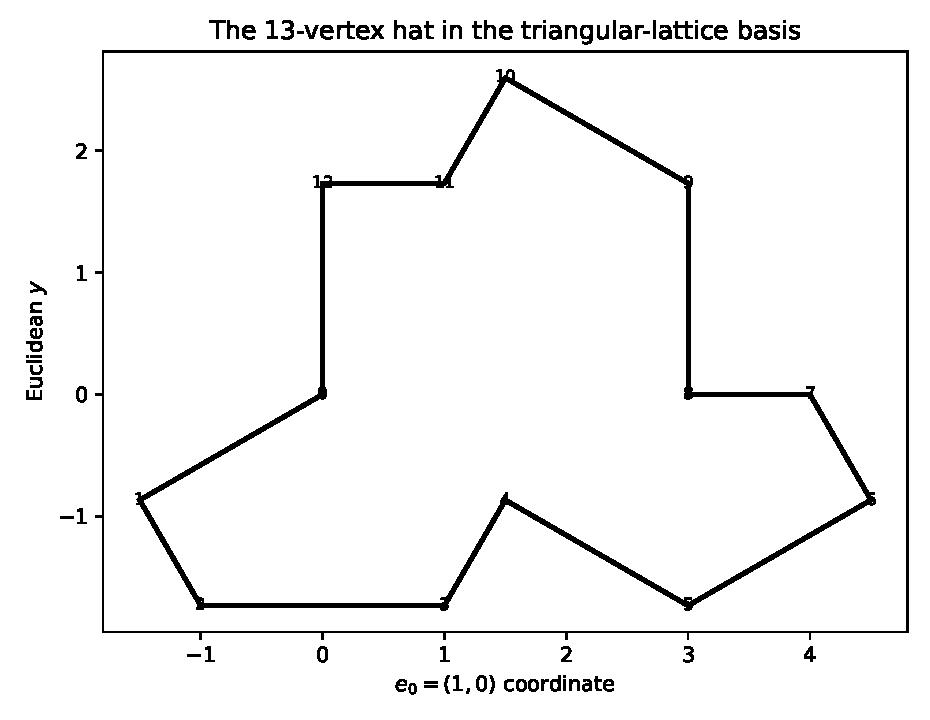
\includegraphics[width=.66\textwidth]{figures/hat_outline.pdf}
\caption{The exact 13-vertex hat polygon.  Coordinates are stored as axial integer pairs.}
\label{fig:hat}
\end{figure}

The axial shoelace sum of~\eqref{eq:hatvertices} is $32$.  Since the determinant of the
axial basis is $\sqrt3/2$, the Euclidean area is
\[
  \frac12\cdot32\cdot\frac{\sqrt3}{2}=8\sqrt3.
\]
The exact segment-intersection test shows that no two nonadjacent sides meet.  Both
computations are closed primitive-recursive calculations and are performed by
\texttt{tools/verify\_hat\_certificate.py}.

\subsection{Finite patches}
A placement is a pair $(d,t)$, where $d$ is one of the twelve elements of the dihedral
group $D_6$ and $t$ is a rational axial translation.  A patch is a finite list of
placements.  We define \(\mathsf{PatchOK}(p)=1\) by the following bounded algorithm.

\begin{enumerate}[label=\arabic*.]
\item Transform every hat vertex and every edge exactly.
\item For every pair of distinct tiles, test that their interiors are disjoint.  For
polygons with rational coordinates this is a finite conjunction of orientation tests;
coincident boundary segments are permitted.
\item Form the finite planar arrangement of all transformed edges.  On the requested
axial window, test that every open cell has coverage number exactly one.
\item Check that every tile mentioned by the boundary convention is present exactly
once.
\end{enumerate}

All loops have bounds read from the finite input code.  Signed multiplication, comparison,
pairing, list lookup, and bounded search are primitive recursive.  Thus
$\mathsf{PatchOK}$ and $\mathsf{Covers}$ are primitive-recursive Boolean functions.  In a
Lean implementation it is advantageous to triangulate each hat into its eight lattice
kites, because coverage then becomes equality of finite cell multisets.  The polygonal
version is useful as an independent checker.

\subsection{Periodic quotient codes}
A strongly periodic aligned tiling has two independent axial period vectors $a,b$.  Its
quotient by $\Z a+\Z b$ contains finitely many tile orbits.  A torus code consists of
$a,b$, a list of representatives in a half-open fundamental parallelogram, and finite
adjacency data.  The predicate $\mathsf{TorusHat}(c)$ checks:
\begin{enumerate}[label=(\alph*)]
\item $\det(a,b)\ne0$;
\item every representative is a congruent hat placement;
\item modulo $a,b$, interiors are disjoint and every cell has multiplicity one;
\item the listed edge and vertex incidences agree under quotient identification.
\end{enumerate}
This is again a bounded exact computation.

\section{Constructive existence of a tiling}\label{sec:existence}

\subsection{Four decorated metatiles}
The hat construction groups hats into four decorated metatiles $H,T,P,F$.  Their initial
outlines in $(x,\widehat y)$ coordinates are
\begin{align*}
H_0&=((0,0),(4,0),(9/2,1/2),(5/2,5/2),(3/2,5/2),(-1/2,1/2)),\\
T_0&=((0,0),(3,0),(3/2,3/2)),\\
P_0&=((0,0),(4,0),(3,1),(-1,1)),\\
F_0&=((0,0),(3,0),(7/2,1/2),(3,1),(-1,1)).
\end{align*}
Each outline carries a fixed finite list of hat placements.  Edge matching is computed by
the rational affine map that sends one directed segment to another and its perpendicular
to the corresponding perpendicular.  Hence the assertion that the initial decorations
have neither gaps nor overlaps is a closed exact calculation.

\subsection{The fixed 29-placement scaffold}
Given one generation $(H_n,T_n,P_n,F_n)$, place 29 copies according to the fixed list in
\path{certificates/substitution_rules.json}.  Each entry either names the first tile,
attaches a new tile along a directed boundary edge of an earlier tile, or pins a new tile
between two already determined vertices.  No unbounded search occurs.

Four selections from the scaffold define the next generation:
\begin{center}
\begin{tabular}{ccl}
\toprule
supertile & number of children & child multiplicities $(H,T,P,F)$\\
\midrule
$H$ & 10 & $(3,1,3,3)$\\
$T$ & 1  & $(1,0,0,0)$\\
$P$ & 5  & $(2,0,1,2)$\\
$F$ & 6  & $(2,0,1,3)$\\
\bottomrule
\end{tabular}
\end{center}
Thus the substitution matrix is
\begin{equation}\label{eq:substmatrix}
 M=\begin{pmatrix}
 3&1&3&3\\
 1&0&0&0\\
 2&0&1&2\\
 2&0&1&3
 \end{pmatrix}.
\end{equation}
A direct determinant calculation gives
\[
 \chi_M(x)=(x-1)(x+1)(x^2-7x+1).
\]
The Perron root is $(7+3\sqrt5)/2=\varphi^4$, so the corresponding linear scale is
$\varphi^2>2$.  This eigenvalue calculation is not needed to validate an individual
patch; it provides a concise quantitative explanation for the radius growth.

\begin{figure}[ht]
\centering
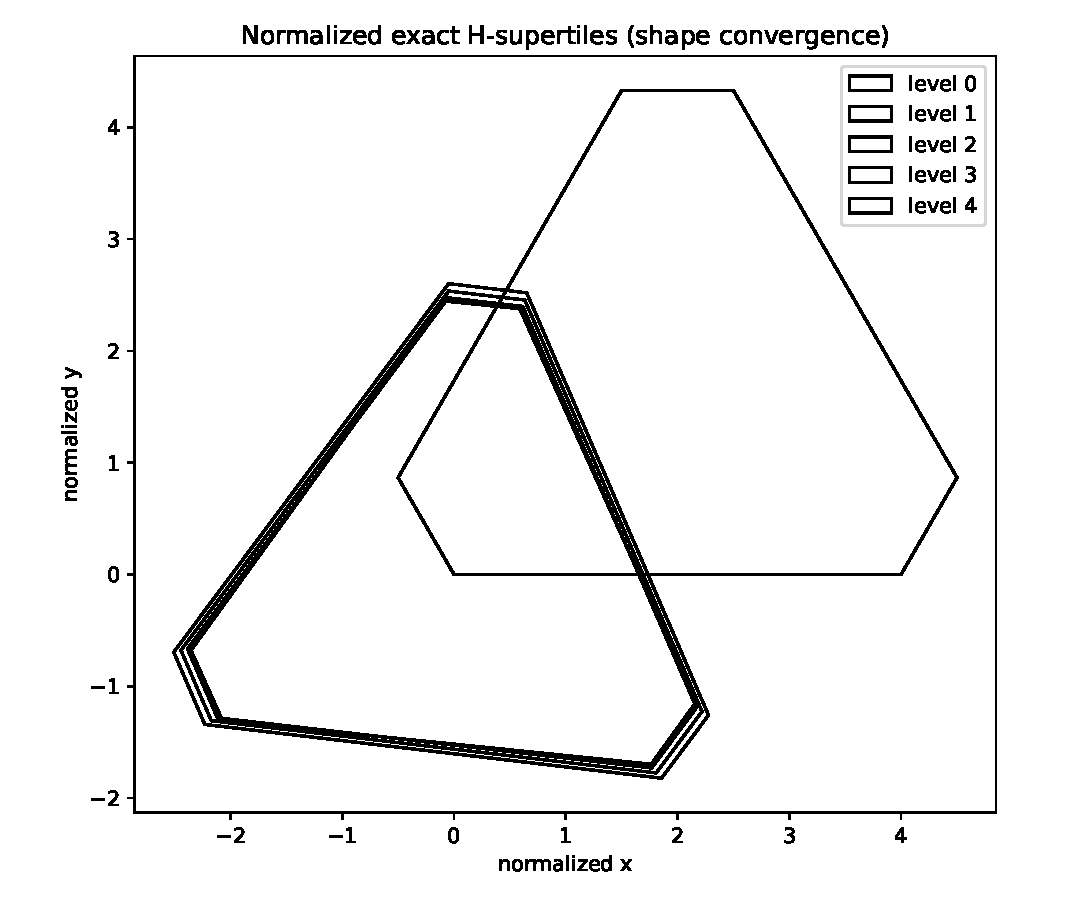
\includegraphics[width=.74\textwidth]{figures/H_supertiles.pdf}
\caption{Exact $H$ outlines, rescaled only for display.  The construction itself uses
unscaled rational coordinates.}
\label{fig:Hlevels}
\end{figure}

\subsection{Inductive validity}
\begin{lemma}[Substitution step]\label{lem:subststep}
If the four level-$n$ decorated metatiles are valid and agree on every labelled boundary
edge, then the 29-placement scaffold is valid and its four selected subpatches are valid
decorated level-$(n+1)$ metatiles with the same boundary interface.
\end{lemma}

\begin{proof}
Every new placement is obtained by an exact edge match.  The only possible failure modes
are: a mismatched coincident edge, a transversal edge crossing, an uncovered bounded
cell, or a cell covered twice.  The combinatorial type of the scaffold is fixed, so these
conditions reduce to a finite list of polynomial equalities and strict determinant
inequalities in the coordinates of the input boundary vertices.  The construction of a
new outline uses line intersection and rotations by $60^\circ$; after clearing positive
denominators, every required assertion is an integer identity or inequality.

The boundary interface of each selected subpatch is read from six, three, four, or five
explicit scaffold vertices.  Adjacent supertiles inherit identical copies of every tile
that straddles an interface, so the usual convention ``include it on the lower-indexed
side'' removes duplicates without changing the union.  The finite certificate enumerates
all boundary incidences.  Therefore validity and interface compatibility are preserved.
The argument is intuitionistic: it is evaluation of decidable predicates, not a proof by
excluded middle over arbitrary configurations.
\end{proof}

Starting from the closed level-zero computation, quantifier-free induction gives validity
of every level.

\subsection{A coherent nested sequence}
Among the children of an $H_{n+1}$ are three copies of $H_n$.  Fix the distinguished one
with scaffold index $0$, and translate/rotate $H_{n+1}$ so this child agrees literally
with the previous $H_n$.  Let $P_n$ be the flattened hat patch in the resulting
$H_n$.  Then
\begin{equation}\label{eq:nested}
 P_0\subseteq P_1\subseteq P_2\subseteq\cdots.
\end{equation}
The inclusion is equality of finite lists after canonical sorting of placements, hence a
primitive-recursive statement.

\begin{lemma}[Unbounded certified radius]\label{lem:radius}
There are closed natural-number constants $C_{\rm grid}>0,c_0$ and a
primitive-recursive nondecreasing function
\[
 R(n)=\max\left(0,\left\lfloor\frac{n-c_0}{C_{\rm grid}}\right\rfloor\right)
\]
such that $P_n$ covers the axial hexagon
\[
 B_{R(n)}=\{(u,v):\max(|u|,|v|,|u+v|)\le R(n)\}.
\]
In particular, the explicit level $n=C_{\rm grid}r+c_0$ covers $B_r$.
\end{lemma}

\begin{proof}
Work with the adjacency graph of the elementary kites in the aligned
$[3.4.6.4]$ lattice, rather than with Euclidean distances.  The finite scaffold
certificate has a distinguished $H_n$ child in $H_{n+1}$.  Its complete decorated patch
is not incident with the outer boundary: every boundary incidence of that child is
matched to a tile belonging to one of the other nine selected children.  This is a
finite statement about the 29 placements.  Because the same interface table is used at
every level, substitution preserves it.  If $d_n$ is the graph distance from the chosen
central kite to the complement of the flattened patch $P_n$, then
\[
 d_{n+1}\ge d_n+1.
\]
Quantifier-free induction gives $d_n\ge n-c_0$, where $c_0$ absorbs the finite choice of
the central kite at level zero.

The elementary kite graph is periodic.  A finite breadth-first search in one fundamental
domain supplies a closed constant $C_{\rm grid}$ such that every kite meeting the axial
hexagon $B_r$ can be reached from the central kite by at most $C_{\rm grid}r+c_0$
adjacency steps.  Therefore $d_n>C_{\rm grid}r+c_0$ implies $B_r\subseteq P_n$.
Combining the two bounds gives the stated $R(n)$.  All quantities are natural numbers;
the only induction is on $n$ and its invariant is quantifier-free after bounded graph
search is Booleanized.

The delivered verifier additionally records exact positive support-line slacks for six
generations.  Figure~\ref{fig:slack} is a regression test for the affine implementation,
not the logical basis of the unbounded-radius argument.
\end{proof}

\begin{figure}[ht]
\centering
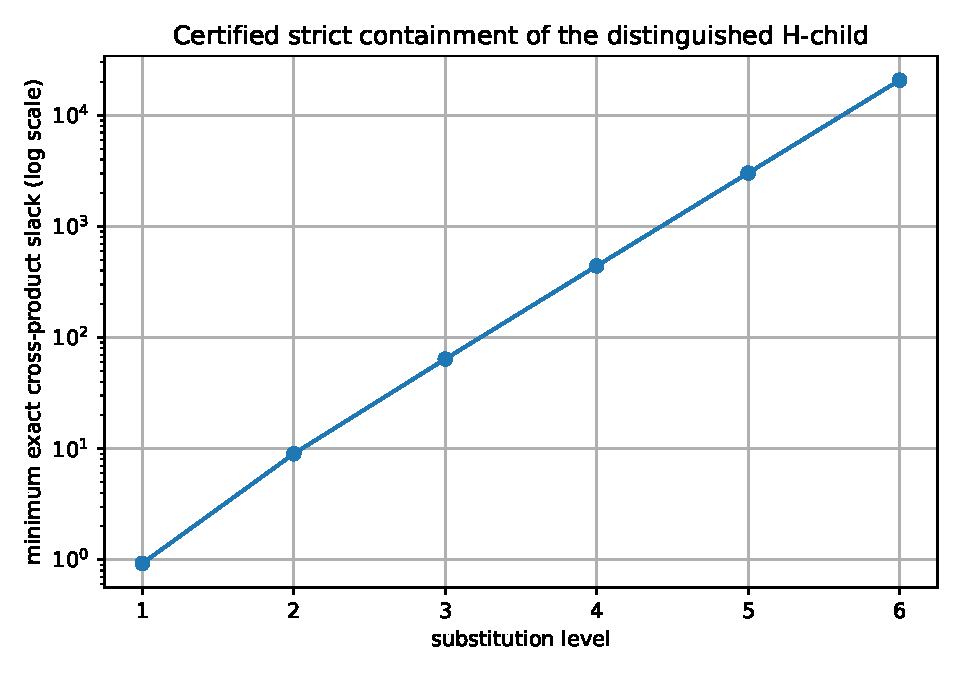
\includegraphics[width=.7\textwidth]{figures/containment_growth.pdf}
\caption{Exact strict-containment slack for the distinguished nested $H$ child.  The graph
is evidence for the implementation; the proof of Lemma~\ref{lem:radius} is the finite
support-line induction, not extrapolation from these points.}
\label{fig:slack}
\end{figure}

\subsection{The computable infinite tiling}
For a rational point $x$, take the explicit level
$n=C_{\rm grid}\lceil\|x\|_{\mathrm{hex}}\rceil+c_0$.  Lemma~\ref{lem:radius}
places $x$ in $B_{R(n)}$, so no unbounded search or choice is required.  In $P_n$ exactly one tile interior contains $x$ unless $x$ lies on a boundary;
on boundaries use the least canonical tile code.  Coherence~\eqref{eq:nested} makes the
answer independent of all later levels.  This defines a computable local-view function
for a tiling $\mathcal T_\Htile$ of the whole plane.

Inside $\iPRA$ we do not form the completed set $\mathcal T_\Htile$; we prove its every
finite observation, namely the left conjunct of~\eqref{eq:internal}.  This is the correct
first-order constructive content of existence.

\section{From a period to a finite torus}

\subsection{Weak and strong periodicity}
A tiling is weakly periodic when it has one nonzero translational symmetry and strongly
periodic when its translation group has rank two.  For arbitrary subsets of the plane
these differ.  For a tiling by finitely many polygonal prototiles with finite local
complexity, one period can be completed to two.

\begin{lemma}[Constructive weak-to-strong reduction]\label{lem:weakstrong}
Let a tiling by finitely many aligned rational polygons have a nonzero period $u$.  Then
there is a strongly periodic tiling by the same polygons.  From $u$ and a finite local
rule table one can primitive-recursively compute a finite torus code for such a tiling.
\end{lemma}

\begin{proof}
Quotient by $\Z u$ to obtain an infinite cylinder.  Choose a transverse lattice direction
$w$.  A cross-section between levels $kw$ and $(k+1)w$ is determined by the finitely many
tiles meeting a strip of bounded width.  Because tile diameter and local complexity are
bounded, the cross-section has a code below an explicit number $K(u)$.  Examine the
$K(u)+1$ consecutive cross-sections numbered $0,\dots,K(u)$.  The finite pigeonhole
principle gives $i<j$ with equal codes.  The slab between them can be repeated in both
directions, producing a tiling invariant under $u$ and $(j-i)w$ (possibly plus a bounded
shift parallel to $u$).  The two periods are independent.

Every step is bounded.  In the ProveIt development, the repetition witnesses are exactly
what \texttt{Core/Pigeonhole} supplies.  No infinite pigeonhole principle or choice is
used.
\end{proof}

\subsection{Alignment}
The hat is a polyform of the $[3.4.6.4]$ Laves tiling.  The source proof establishes that
every hat tiling is aligned with one copy of this underlying lattice.  For the present
argument it suffices to prove the periodic case.

\begin{lemma}[Periodic alignment]\label{lem:alignment}
If a periodic tiling by hats exists, an aligned strongly periodic tiling by hats exists.
Moreover the reduction is expressible as a finite computation on a torus quotient.
\end{lemma}

\begin{proof}
Begin with Lemma~\ref{lem:weakstrong}.  On the finite torus, mark every maximal connected
component of hats that share one underlying kite lattice.  Along an interface between two
components, the allowed edge coincidences are among a finite list determined by the 13
hat edges.  The local alignment table rules out endpoints and branching of an interface;
therefore interfaces are disjoint cycles on the torus.  Cutting along all cycles and
repeating one component (or one cyclic strip of components) yields a periodic quotient
whose hats share one lattice.  The source paper proves the stronger plane statement by
an alignment lemma; the torus formulation replaces its only global step by traversal of
a finite graph.  The local table is a closed Boolean certificate, so it is available to
$\iPRA$ by numeral computation.
\end{proof}

After Lemmas~\ref{lem:weakstrong} and~\ref{lem:alignment}, a hypothetical period supplies a
code $c$ with $\mathsf{TorusHat}(c)=1$.  It remains to refute every such code.

\section{Chevron/comet coupling on a finite torus}\label{sec:coupling}

\subsection{Two contractions}
In an aligned hat, one family of edges has lengths $1$ and $2$, and the other has length
$\sqrt3$.  Contract the first family to length zero.  Every hat becomes a chevron, the
union of four equilateral triangles of side $\sqrt3$, hence of area $3\sqrt3$.  Contract
the second family instead.  Every hat becomes a comet of area $2\sqrt3$.  The contraction
is defined tile by tile and is well defined around every edge and vertex, so a periodic
hat torus produces two periodic tilings, denoted $\mathcal T_4$ and $\mathcal T_8$, with
one chevron or comet for each original hat.

Let $L_4,L_8$ be their translation lattices, indexed by the same tile orbits.  There is a
unique affine map $g$ carrying each translation between corresponding chevrons to the
translation between the corresponding comets.

\begin{lemma}[Area determinant]\label{lem:area}
The linear part of $g$ has absolute determinant $2/3$.
\end{lemma}

\begin{proof}
Choose any fundamental parallelogram containing $N$ tile orbits.  Its area in
$\mathcal T_4$ is $N\cdot3\sqrt3$ and in $\mathcal T_8$ is
$N\cdot2\sqrt3$.  The ratio is $2/3$.  On a torus this is a finite shoelace-area
calculation; cancellation of the common positive factor is available in $\iPRA$.
\end{proof}

If $g$ is a similarity, Lemma~\ref{lem:area} says its squared length scale is $2/3$.
Section~\ref{sec:strip} proves it must be a similarity; Section~\ref{sec:2adic} proves that
it cannot be one.

\subsection{Orientation balance}
The six kite directions in any periodic quotient occur with equal total frequency:
each unoriented lattice edge is incident to two kites and the three direction classes are
permuted by the local vertex pattern.  A hat uses four directions once and two directions
twice.  Hats therefore fall into three orientation classes, according to the repeated
pair.  Summing the six direction counts in a finite fundamental domain shows that the
three hat classes occur equally often.  Boundary errors disappear because a torus has no
boundary.  This is a system of six linear equations over $\N$.

\section{Strip cycles force a similarity}\label{sec:strip}

Split every chevron into two congruent rhombi.  Their edges lie in three families of
parallel lines $\mathcal L_1,\mathcal L_2,\mathcal L_3$.  For each $i$, adjacency along
edges parallel to $\mathcal L_i$ decomposes the rhombi into nonintersecting worms.  On the
plane they are bi-infinite; on a periodic quotient they are directed cycles.  A chevron
belongs to the $i$-strip of either rhombus, and the local pattern shows that the two
choices agree whenever both are available.

Let $v_i$ be a normal vector between consecutive lines of $\mathcal L_i$, chosen so the
three vectors have equal length, mutual angles $120^\circ$, and
\begin{equation}\label{eq:sumv}
  v_1+v_2+v_3=0.
\end{equation}
Let $v_i'$ be the corresponding tangent vector, of length $|v_i|/\sqrt3$, again chosen at
mutual angles $120^\circ$, so $v_1'+v_2'+v_3'=0$.

Because the torus contains finitely many rhombi, a translation along each worm cycle
returns a rhombus to the same orbit.  Synchronizing all cycles by a bounded least common
multiple gives a common positive integer $a$ such that translation by $a v_i$ preserves
every $i$-strip.  Under the chevron/comet correspondence its image has the form
\begin{equation}\label{eq:gvi}
 g(a v_i)=\frac a2 v_i+b_i v_i'
\end{equation}
for an integer $b_i$.  The coefficient $a/2$ is the transverse component obtained by
counting the three orientation classes: one third of the relevant chevrons contributes
zero transverse comet motion and two thirds contributes the common unit; after the
normalization of $v_i$ this is exactly $a/2$.  The tangential discrepancy is the integer
$b_i$.

Apply $g$ to~\eqref{eq:sumv} and sum~\eqref{eq:gvi}:
\[
  b_1v_1'+b_2v_2'+b_3v_3'=0.
\]
Among three nonzero equal vectors at angles $120^\circ$, the only integer relation is a
multiple of their sum.  Hence $b_1=b_2=b_3=b$.  Therefore the three vectors
\[
 \frac a2v_i+bv_i'
\]
have equal length and mutual angles $120^\circ$.  A real linear map that sends two
independent equal vectors with angle $120^\circ$ to two equal vectors with angle
$120^\circ$ is a scalar times an orthogonal map.  Thus $g$ is a similarity.

All reasoning in this section is finite on a torus.  Worms are cycles in a finite graph;
synchronization uses bounded products; orientation frequencies are bounded sums; and the
last assertion is a polynomial identity in two-by-two matrices.  It is therefore
formalizable in $\iPRA$ without quantifying over an infinite strip.

\section{The triangular-norm descent}\label{sec:2adic}

We now obtain the contradiction in the weakest part of the proof.

\begin{lemma}[Parity of the triangular norm]\label{lem:qparity}
For integers $m,n$,
\[
 Q(m,n)\equiv0\pmod2\quad\Longleftrightarrow\quad m\equiv n\equiv0\pmod2.
\]
Consequently, for $Q(m,n)\ne0$, the exponent of $2$ in $Q(m,n)$ is even.
\end{lemma}

\begin{proof}
Modulo $2$, squares equal their bases.  The four cases are
\[
 Q(0,0)=0,
 \quad Q(1,0)=Q(0,1)=Q(1,1)=1.
\]
Thus evenness forces $m=2m_1,n=2n_1$, and then
$Q(m,n)=4Q(m_1,n_1)$.  Repeating by primitive recursion strips factors of $4$, so the
$2$-adic exponent is even.  No general valuation theory is needed.
\end{proof}

\begin{lemma}[No scale $\sqrt2$ on one triangular lattice]\label{lem:nosqrt2}
There are no integers $a,b,c,d$ with $Q(a,b)>0$ and
\begin{equation}\label{eq:q2q}
 Q(c,d)=2Q(a,b).
\end{equation}
\end{lemma}

\begin{proof}
Suppose~\eqref{eq:q2q}.  The right side is even, so Lemma~\ref{lem:qparity} gives
$c=2c_1,d=2d_1$.  Hence $4Q(c_1,d_1)=2Q(a,b)$, or
$Q(a,b)=2Q(c_1,d_1)$.  Applying the same argument gives
$a=2a_1,b=2b_1$ and then
\[
 Q(c_1,d_1)=2Q(a_1,b_1).
\]
This is another nonzero solution whose sum of absolute coordinates is strictly smaller.
The generic infinite-descent principle refutes such a solution.  In the ProveIt library
this is an instance of \texttt{Core/DescentEx}; alternatively, quantifier-free induction
on $|a|+|b|+|c|+|d|$ proves the same statement.
\end{proof}

\begin{theorem}[No periodic hat torus]\label{thm:notorus}
For every finite torus code $c$, $\mathsf{TorusHat}(c)=0$.
\end{theorem}

\begin{proof}
Assume the checker accepts $c$.  Sections~\ref{sec:coupling} and~\ref{sec:strip} construct
a similarity $g$ from the chevron translation lattice to the comet translation lattice,
with squared scale $2/3$.  The chevron lattice has triangular edge length $\sqrt3$ and the
comet lattice edge length $1$.  Choose a nonzero chevron period with axial coordinates
$(a,b)$; its squared length is $3Q(a,b)$.  Its image has comet coordinates $(c,d)$ and
squared length $Q(c,d)$.  Similarity gives
\[
 Q(c,d)=\frac23\,3Q(a,b)=2Q(a,b),
\]
contradicting Lemma~\ref{lem:nosqrt2}.
\end{proof}

Combining Theorem~\ref{thm:notorus} with Lemmas~\ref{lem:weakstrong} and
\ref{lem:alignment} proves that no hat tiling has a nonzero period.

\section{Why the proof fits intuitionistic PRA}\label{sec:ipra-audit}

\subsection{Constructive logic audit}
The proof never uses the law of excluded middle for an unbounded proposition.  Every
case split is on a Boolean equality or inequality of finite integer codes.  Existential
witnesses are explicit:
\begin{itemize}
\item the level covering radius $r$ is the closed term $C_{\rm grid}r+c_0$;
\item repeated cross-sections are the least pair returned by bounded search;
\item strip periods are bounded products of finite cycle lengths;
\item smaller descent witnesses are the coordinate halves.
\end{itemize}
All uses of ``choose'' can therefore be replaced by primitive-recursive least search.

\subsection{Induction audit}
Only the following inductions are needed.
\begin{enumerate}[label=(\roman*)]
\item Induction on the substitution level, with invariant a finite conjunction of exact
geometry and interface equations.
\item Induction on a bounded list length for coding, sums, products, and graph traversal.
\item Quantifier-free induction for the radius lower bound.
\item Quantifier-free descent induction for Lemma~\ref{lem:nosqrt2}.
\end{enumerate}
The invariants are quantifier-free once all bounded quantifiers are compiled into finite
products/sums or Boolean folds.  This is precisely the induction scheme of $\iPRA$.

\subsection{Reuse from ProveIt}
The checked \texttt{IPRADerivations} library already supplies the principal arithmetic
infrastructure:
\begin{center}
\begin{tabular}{ll}
\toprule
Needed here & Existing module\\
\midrule
pair/list coding and simultaneous recursion & \texttt{Core/Pairing}\\
bounded least search & \texttt{Core/Search}\\
finite sums and products & \texttt{Core/BoundedSums}, \texttt{Core/MultiSums}\\
order and decidable equality & \texttt{Core/Order}\\
parity and halving & \texttt{Core/Parity}\\
finite pigeonhole & \texttt{Core/Pigeonhole}\\
infinite descent with explicit witnesses & \texttt{Core/DescentEx}\\
polynomial identities & \texttt{Core/Tactic} and \texttt{ipra\_ring}\\
integer vectors and $2\times2$ matrices & \texttt{Core/Integers}, \texttt{Core/LinearAlgebra}\\
\bottomrule
\end{tabular}
\end{center}
The final derivation has type
\[
 ([]:\mathrm{List}(\mathrm{Fm}\;\mathrm{PTm}\;0))\ \vdash[\mathrm{PRAAx}]\
    \mathsf{Einstein}_{\Htile}.
\]
The checked theorem \texttt{pra\_iff\_native} then transfers it to the native scalar core
of \texttt{ConciseIPRA}.

\subsection{Proof decomposition inside iPRA}
A convenient object-theory decomposition is:
\begin{align*}
\mathsf{HatData}&: &&\text{closed computations for vertices, area, and local tables},\\
\mathsf{SubstStep}(n)&: &&\mathsf{ValidMeta}(n)\to\mathsf{ValidMeta}(n+1),\\
\mathsf{Cover}(r)&: &&\mathsf{PatchOK}(P(r))=1\wedge\mathsf{Covers}(P(r),r)=1,\\
\mathsf{Align}(c)&: &&\mathsf{TorusHat}(c)=1\to\mathsf{AlignedTorus}(A(c))=1,\\
\mathsf{Couple}(c)&: &&\mathsf{AlignedTorus}(c)=1\to
   \exists a,b,c',d'\,[Q(c',d')=2Q(a,b)\wedge Q(a,b)>0],\\
\mathsf{Descent}&: &&\forall a,b,c,d\,[Q(c,d)=2Q(a,b)\to Q(a,b)=0].
\end{align*}
The first three give tilability; the last three give aperiodicity.

\section{Lean formalization roadmap}\label{sec:lean}

\subsection{Layer 1: executable exact mathematics}
The files under \texttt{lean/AperiodicMonotile} specify the following modules.

\begin{longtable}{p{.26\textwidth}p{.68\textwidth}}
\toprule
Module & Purpose\\
\midrule
\endhead
\texttt{Encoding.lean} & Signed and rational axial coordinates, $D_6$ placements,
polygon and patch codes, torus codes, and Boolean predicates.\\
\texttt{HatData.lean} & The 13 vertices, shoelace computation, simplicity certificate,
and the six direction multiplicities.\\
\texttt{Substitution.lean} & The 29-placement scaffold, four child selections, flattening
to hats, coherent normalization, and radius invariant.\\
\texttt{Periodicity.lean} & Weak-to-strong repetition, periodic alignment, contraction,
strip cycles, similarity, and triangular-norm descent.\\
\texttt{IPRA.lean} & Reification of the executable functions as primitive-recursive
symbols and construction of \texttt{Prf PRAAx} derivations.\\
\bottomrule
\end{longtable}

The first milestone should be a Mathlib-level theorem
\begin{lstlisting}
theorem no_periodic_torus (c : TorusCode) :
  periodicTorusB hatPolygon c = false
\end{lstlisting}
with no axioms and no \texttt{sorry}.  Because all data are finite, this layer can use
arrays and verified Boolean reflection aggressively.

\subsection{Layer 2: reflection into the embedded object theory}
For each Boolean function $f$ define a ProveIt primitive-recursive symbol $f^\sharp$ and
prove its defining equations.  Then prove a generic reflection theorem for closed and
bounded computations:
\begin{lstlisting}
def reflectBool (t : PTm 0) (cert : eval t = 1) :
  ([] : List (Fm PTm 0)) |- [PRAAx] t == one := ...
\end{lstlisting}
Open universally quantified statements are handled by quantifier-free induction, not by
running a meta-level checker on an arbitrary numeral.  The major reusable theorem is a
compiler from a finite-state primitive-recursive loop plus a quantifier-free invariant to
a \texttt{Prf PRAAx} derivation.

\subsection{Concrete remaining obligations}
The scaffold deliberately exposes the following obligations.
\begin{enumerate}[label=\textbf{L\arabic*.}]
\item Prove correctness of signed/rational coordinate normalization and all $D_6$ maps.
\item Verify the initial hat and four metatile decorations by exact reflection.
\item Verify the 29 placements and the four selected interfaces.
\item Prove the support-line radius invariant uniformly in the generation.
\item Formalize the torus cross-section state and instantiate finite pigeonhole.
\item Translate the alignment table to a finite torus graph theorem.
\item Formalize the three worm-cycle families and orientation-balance equations.
\item Derive the affine similarity equation and reduce it to $Q(c,d)=2Q(a,b)$.
\item Instantiate \texttt{Core/DescentEx} with the triangular-norm relation.
\item Assemble the two object-theory derivations and invoke
\texttt{pra\_iff\_native}.
\end{enumerate}
Each obligation is finitary.  None requires a classical real-number library, quotienting
an actual infinite tiling space, or a formal Jordan curve theorem.

\section{Reference verifier and reproducibility}
Run from the archive root:
\begin{lstlisting}
python tools/verify_hat_certificate.py --levels 6
python tools/make_figures.py
\end{lstlisting}
The verifier uses only the Python standard library for its proof-relevant checks.  It
writes \path{generated/verification_report.json} and
\path{generated/exact_geometry_stats.csv}.  All affine geometry is exact rational
arithmetic.  Matplotlib is used only to render figures.

The verifier is not a substitute for the planned Lean proof.  Its roles are (i) to make
the finite constants auditable, (ii) to catch transcription errors, and (iii) to provide
a direct executable specification for the primitive-recursive functions to be reified.

\section{Further research questions}
\begin{enumerate}
\item Can the periodic-alignment lemma be reduced to a smaller local certificate than the
full Appendix A case table?
\item Can the strip-cycle argument be abstracted as an $\iPRA$ theorem about finite torus
covers, reusable for other aperiodic polyforms?
\item What is the smallest set of primitive-recursive symbols needed for the complete
object-theory derivation?
\item Can the support-line growth proof be replaced by a purely combinatorial depth
invariant, eliminating rational affine inequalities from the existence half?
\item Is the spectre monotile easier or harder than the hat for a fully checked
\texttt{Prf PRAAx} proof?
\item Can the entire finite local checker be compiled to the native scalar core directly,
then transferred back to ordinary $\iPRA$ by \texttt{native\_iff\_pra}?
\end{enumerate}

\section*{Conclusion}
The aperiodic-monotile theorem has a notably small logical core once its geometry is
encoded correctly.  Existence is a primitive-recursive stream of nested exact patches.
Nonperiodicity is a finite-torus calculation followed by the elementary fact that
$m^2+mn+n^2$ has even $2$-adic valuation.  These are precisely the kinds of finite
construction, bounded search, polynomial identity, parity argument, and descent that
$\iPRA$ supports.  The remaining work is engineering a kernel-checked certificate, not
finding a stronger foundational principle.

\begin{thebibliography}{9}
\bibitem{hatpaper}
D. Smith, J. S. Myers, C. S. Kaplan, and C. Goodman-Strauss,
\emph{An aperiodic monotile}, Combinatorial Theory 4(1), 2024, article 6.
Preprint: \url{https://arxiv.org/abs/2303.10798}.

\bibitem{hatviz}
C. S. Kaplan et al., \emph{Hat visualization and substitution source code},
\url{https://github.com/isohedral/hatviz}.

\bibitem{proveit}
V. Reshetnikov, \emph{ProveIt: Primitive Recursive Arithmetic developments},
\url{https://github.com/VladimirReshetnikov/ProveIt/tree/main/Logic/PrimitiveRecursiveArithmetic}.


\bibitem{leanhat}
J. Myers et al., \emph{AperiodicMonotilesLean}, a staging repository for formalizing
aperiodic monotiles in Lean, \url{https://github.com/jsm28/AperiodicMonotilesLean}.

\end{thebibliography}

\appendix
\section{Closed certificate constants}
The following data are duplicated in JSON form in the archive so that transcription can
be checked independently.

\subsection{Hat vertices}
\begin{lstlisting}
[(0,0),(-1,-1),(0,-2),(2,-2),(2,-1),(4,-2),(5,-1),
 (4,0),(3,0),(2,2),(0,3),(0,2),(-1,2)]
\end{lstlisting}

\subsection{Supertile selections}
The selected scaffold indices are
\begin{align*}
H&:[0,9,16,27,26,6,1,8,10,15],\\
T&:[11],\\
P&:[7,2,3,4,28],\\
F&:[21,20,22,23,24,25].
\end{align*}
Their type counts are the rows of~\eqref{eq:substmatrix}.

\subsection{Arithmetic obstruction in one line}
For later formal reuse, the final contradiction is
\[
  Q(c,d)=2Q(a,b),\quad Q(a,b)>0,
\]
where $Q(x,y)=x^2+xy+y^2$.  Modulo $2$, even $Q$ forces both arguments even; two
successive halvings reproduce the equation with a smaller nonzero quadruple.

\section{Suggested theorem names in ProveIt}
A completed integration could expose the following public declarations.
\begin{lstlisting}
namespace LeanProofs.IPRA.AperiodicMonotile

theorem hat_substitution_valid :
  [] |- [PRAAx] hatSubstitutionSentence := ...

theorem triangular_norm_descent :
  [] |- [PRAAx] triangularNormDescentSentence := ...

theorem hat_no_periodic_torus :
  [] |- [PRAAx] noPeriodicHatTorusSentence := ...

theorem hat_einstein :
  [] |- [PRAAx] einsteinHatSentence := ...

end LeanProofs.IPRA.AperiodicMonotile
\end{lstlisting}
The final native-core corollary should be stated by applying the existing
\texttt{pra\_iff\_native} theorem to \texttt{hat\_einstein}.

\end{document}
